\chapter{Data compression}\label{textcompr}

	This thesis was submitted at Czech Technical University in Prague (see Figure~\ref{fig:logo}).
	
	\begin{figure}\centering
		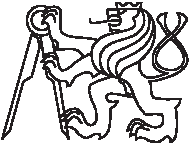
\includegraphics{figures/cvut-logo-bw}
		\caption{CTU logo}\label{fig:logo}
	\end{figure}

\section{Notions and definitions}

The source \textit{message} consists of \textit{source units}, which can be defined as \textit{alphabet symbols} or sequence of alphabet symbols \textit{(word, string, phrase)}, where alphabet $S$ is a finite and non-empty set of symbols. The \textit{code unit} is defined as a sequence of bits. The empty sequence of symbols is called \textit{empty string} and it is represented by $\varepsilon$. The set of all symbols from alphabet $S$, free of empty string, is represented by $S^+$. The \textit{concatenation} of two phrases $x,y \in S$ is represented by $x.y$.

Code is a triple $K=(S,C,f)$, where

\begin{itemize}
	\item $S$ is a finite set of source units,
	\item $C$ is a finite set of codewords (code units),
	\item $f$ is an injective mapping from $S$ to $C^+$.
\end{itemize}
The mapping $f$ does not map two different source units from $S$ to the same codeword from $C$, as shown Formula \ref{eq:injectionf}.
\begin{equation} \label{eq:injectionf}
\forall a_1,a_2 \in S,a_1 \neq a_2 \Rightarrow f(a_1) \neq f(a_2)
\end{equation}
The string $x \in C^+$ is \textit{uniquely decodable} with $f$, when Formula \ref{eq:unadec} is true.
\begin{equation} \label{eq:unadec}
\forall y_1,y_2 \in S^+,f(y_1)=f(y_2)=x \Rightarrow y_1=y_2
\end{equation}

The code $K=(S,C,f)$ is \textit{uniquely decodable}, when all strings $x \in C^+$ are uniquely decodable  in $f$. The code $K$ is called \textit{prefix code}, when none of codewords is a prefix of another codeword. If all codewords are exactly $n$ symbols length in code $K$, the code $K$ is called \textit{block code}. The prefix codes and block codes are often used by compression algorithms because of their unique decode-ability during the left-to-right reading (decoding).

\begin{equation} \label{eq:comrat}
\textrm{\textit{Compression ratio}} = \frac{\textrm{\textit{Length of compressed data}}}{\textrm{\textit{Length of original data}}}
\end{equation}

The compression efficiency can be expressed by many units of measure. The amount of data reduction gained by the compression process is \textit{compression ratio}. This compression ratio is a ratio of the length of compressed data to the original size of data (Formula \ref{eq:comrat}).
For example, the compression ratio is measured in $bpb$ (bits per bit), $bpc$ (bits per character) or $bpp$ (bits per pixel). 

The compression algorithms use specific \textit{compression models} to encode the data. For example, these models could follows:
\begin{itemize}
	\item The algorithm assigns code to each source unit irrespective to its position (statistical compression methods).
	\item The Markov's model of $n$-th order look at previous $n$ source units to assign code. The simplist of this codes, 0th order, are mentioned above.
	\item The models based on finite automata.
\end{itemize}

	\subsection{Entropy}
The entropy is only theoretical minimal length but it is possible to reach this border in some special cases. It is very difficult to measure real entropy of source message in common usage, because not only statistical model of 0th order (context of source units with length 1) exists. For example, the probabilities of appearances of source units pairs (context of source units with length 2) are considered in 1st order statistical model. 

	\subsection{Classification}

Data compression/decompression is classified by many factors. The first classification depends on information loss during the compression process. The data compression, as data compression algorithms, is divided into two main parts:
\begin{itemize}
	\item \textit{Lossy}---some information loss is possible. These compression methods achieve higher compression (better compression ratio) but they are useful only in special cases (images, video, voice...).
	\item \textit{Lossless}---information is acquired in original form. These compression methods are best suited for data where loss is unacceptable (documents, programs, scripts...).
\end{itemize}

\section{Elementary methods}

Many elementary compression methods are currently known, but only the \gls{RLE} is mentioned on as very simple compression method, to show how compression methods work.

	\subsection{RLE}
The \gls{RLE} technique was created especially for data with strings of repeated symbols (the length of string of repeated symbols is called \textit{run}). The main idea of \gls{RLE} compression is to encode repeated symbols as a pair---the length of string and the symbol.

\begin{table}\centering
	\caption{RLE example}\label{tab:RLE-example}
	\begin{tabular}{|c|r|r|}
	\hline \textbf{Method} & \textbf{Data to encode} & \textbf{Encoded data} \\\hline
	RLE 1 & \textit{babaaaaabbbaabbbba11aaa} & \textit{$1$b$1$a$1$b$5$a $3$b$2$a$4$b$1$a $2$1$3$a} \\\hline
	RLE 2 & \textit{babaaaaabbbaabbbba11aaa} & \textit{bab$@5$a$@3$ baa$@4$ba1 1$@3$a} \\\hline
	\end{tabular}
\end{table}

There are shown some ways of \gls{RLE} compression of 23-characters-long string \textit{``babaaaaabbbaabbbba11aaa''} in Table \ref{tab:RLE-example}. The first method (RLE 1) is the simplest way to encode string (20 characters) which exactly follows idea of \gls{RLE}. The problem is that in worst case the size of output data can be two times longer than size of input data. This problem is solved by second method (20 characters), for simplicity called RLE 2, where only three or more characters long strings are encoded, but we pay for it by another character (\textit{$@$} in example), which precede all of encoded pairs, to differentiate between the length of string and the number as a character. The third method (RLE 3) solves this problem by map of bits (18~characters). \gls{RLE} compression method is very useful for graphic files coding but it is practically useless in text compressions without using it cooperatively with other methods.

%\section{Statistical methods}


\section{Dictionary methods}

	\subsection{LZ77}
It is obvious that the value of offset and the match length have to be limited to some constant. The usually chosen value for the match length is 255 (8~bits) and the offset is commonly encoded on 12--16 bits, so the search buffer is limited to 4~095--65~535. In so far that there is no need to remember more than 65 535 already encoded symbols during compression process.
